% This is based on the LLNCS.DEM the demonstration file of
% the LaTeX macro package from Springer-Verlag
% for Lecture Notes in Computer Science,
% version 2.4 for LaTeX2e as of 16. April 2010
% 
% See http://www.springer.com/computer/lncs/lncs+authors?SGWID=0-40209-0-0-0
% for the full guidelines.
%
\RequirePackage{fix-cm}
%
%\documentclass{svjour3}                     % onecolumn (standard format)
%\documentclass[smallcondensed]{svjour3}     % onecolumn (ditto)      % onecolumn (second format)
%\documentclass[twocolumn]{svjour3}          % twocolumn
%
%

\documentclass{llncs}
\usepackage{graphicx}
\begin{document}

\title{Goal Trajectories for Knowledge Investigations}
%
\titlerunning{Hamiltonian Mechanics}  % abbreviated title (for running head)
%                                     also used for the TOC unless
%                                     \toctitle is used
%
\author{Vahid B. Eyorokon \and Benjamin Bengfort\inst{2}
\and Uday S. Panjala \and Michael T. Cox}
%
\authorrunning{Ivar Ekeland et al.} % abbreviated author list (for running head)
%
%%%% list of authors for the TOC (use if author list has to be modified)
\tocauthor{Ivar Ekeland, Roger Temam, Jeffrey Dean, David Grove,
Craig Chambers, Kim B. Bruce, and Elisa Bertino}
%

\institute{Wright State University, Dayton OH 45435, USA\\
\email{michael.cox@wright.edu},\\ WWW home page:
\texttt{http://mcox.org}
\and
University of Maryland,
College Park, MD 20742, USA}

 
\maketitle              % typeset the title of the contribution

\begin{abstract}
Humans seek to gain knowledge and structure data by many means including both bottom-up and top-down methods. But in most instances, people have a specific purpose to their activity with data that drives the process. They often have particular questions that need answering in support of some broader investigation. These questions often change as answers point in various directions during an investigation, whether the investigation is formal (e.g., scientific, legal, journalistic, or military) or simply an informal browsing of the internet. In this paper, we take a mixed-initiative approach to knowledge discovery, and we present a system called Kyudo that supports the process using a conversational case-based reasoning process. Cases in Kyudo are sequences of knowledge goals or questions that form arcs through a multidimensional knowledge space and that form the core activity in a dialogue between the user and system. As the system gains more experience and therefore more cases, it is able to detect similarity in knowledge goals and prompt the user with additional relevant goals that can short circuit the human reasoning process to minimize tangents or false starts. In this paper we present a distance-based mechanism that reduces the total length of a goal trajectory through guidance that accelerates the human reasoning process and aids effective knowledge discovery.
\keywords{Case-based reasoning, goal trajectories, knowledge goals, goal guidance, knowledge discovery}
\end{abstract}
%
\section{Introduction}
%
Information retrieval and knowledge discovery systems using statistical inference mechanisms have changed the way we interact with data. Search techniques have evolved to allow the parsing of natural language questions into a structured database query \cite{yahya_natural_2012} or lambda calculus representation \cite{berant_semantic_2013} that can be executed against a structured knowledge base. This has resulted in a shift in the balance between the amount of work a human has to do to answer questions or perform a query and the amount of work of a cognitive augmentation system. For example previous search techniques were designed to deliver the most relevant content to a human user, but left them the task of reading and interpreting that content to inform their specific goals.

	Now, because human users can get immediate, automated responses to fact oriented questions including superlative and aggregation questions (e.g., ``which country has the most gold medals per capita?'') the focus has shifted to higher level queries, particularly those that require creativity like explanation or associative queries. Here we view such queries as an investigative goal, more specifically a \textit{knowledge goal} \cite{bengfort_interactive_2015,ram_1990,ram_1991}. Knowledge goals are structures that represent an agent's desires for knowledge and often are expressed naturally as natural language questions. These types of knowledge goals require a research or investigative approach to reasoning, where an initial goal changes throughout the course of solving the goal because of new information and increasing precision. Therefore we can say that the act of investigation necessarily involves the creation of a \textit{knowledge goal trajectory}, where the posing of an initial knowledge goal is refined, focused, or changed through a variety of phases in the investigative sequence, usually in a creative manner as a reaction to information retrieved with factual sub-goals that can be quickly retrieved to confirm or reject hypotheses or assumptions that led to the initial goal.

	Because of the creative elements of this type of reasoning, crowd-sourcing has become a popular approach for investigation \cite{wang_wisdom_2013}. Instead, we propose a mixed-initiaitve, case-based reasoning system where humans propose their investigations in the form of \textit{dialogues}. As such a case represents a sequence of questions posed to the system together with its associated retrievals. The underlying case-based reasoning system provides guidance to the user by retrieving previous cases that illustrate the investigative process. By representing knowledge goals as a multidimensional vector of semantic features, we can compute the distance between knowledge goals in a semantic space and thus find similar cases. As users interact with the system, the total goal distance can be computed as the length of the path of  goals from the initial to final goals of the dialogue. If a system is able to recommend goals by reusing previous cases that decrease the length of the goal trajectory, or simply short circuit tangents or bad investigative paths, then it can be said to be providing guidance and augmenting the cognitive aspects of investigation for a human user.

	We first present an interactive, mixed-initiative knowledge goal reasoning system that leverages cased-based reasoning to provide guidance to a user inside of an investigative dialogue. We then describe our goal vectorization methodology in detail as well as the algorithm that provides guidance to the user in goal space. Next, we will describe the retrieval and analysis of contextually, conceptually and task related cases. Finally, we will present related research and conclude.
%
\section{Case-based Reasoning for Knowledge Trajectories}
%

Our proposed approach for complex knowledge goal reasoning is a \textit{case-based reasoning} (CBR) \cite{kolodner_case-based_1993,lopez_de_mantaras_retrieval_2005} system called Kyudo\footnote{The way of the bow, is a Japanese martial art of archery. The idea of goal trajectories to solve knowledge goals is much like the flight of an arrow to hit a target.} \cite{bengfort_interactive_2015} which reuses past experience in an interactive fashion. Interactive CBR operates similarly to conversational case-based reasoning systems, which incrementally elicits a target problem through an interactive dialog with the user, attempting to minimize the number of questions before a solution is reached \cite{aha_advances_2005}. To provide an adaptable, investigative system, the methodology we are exploring guides the user in a finite length interactive dialogue, removing the requirement to minimize session length to facilitate an ongoing discovery process. Additionally, the system itself is a learning agent with the goal of predicting future knowledge goals, and acquiring the information in advance to provide specific guidance to the user.
%
\subsection{Goal Trajectories}
%
In interactive knowledge-goal reasoning, a complex knowledge goal is broken down into a hierarchical plan involving simpler sub-goals and tasks to augment the investigative process of a user. During an investigative dialogue, the user selects the next step of plans proposed by the reasoner, and continues to chain sub-goals together to work towards a larger solution. During this process, the plan is adaptable and subject to change as the user proceeds in selecting and executing the simpler goals. Goals, like plans, are also subject to change and can be transformed \cite{cox_goal_1998}, therefore we propose that the original knowledge goal itself is also subject to change; and that as knowledge goals change during interactive reasoning, the path that led to the solution of new goals from the original can be represented by a \textit{goal trajectory}.

	Goal trajectories can be influenced either through the direct interactive manipulation of goals \cite{cox_mixed-initiative_2007}; via other users in the system issuing similar queries that provide the basis for recommending new goals; or by the monitoring of new information or relevant data that has been added to the knowledge base. An investigative dialogue can be therefore seen as a planning problem where knowledge goals are not static and must be responsive to goal changes. We believe that a system can leverage goal change to provide guidance by proposing medium steps towards a series of predicted goals. This guidance will accelerate the user who is likely to take short steps toward a goal, yet not provide uncanny or mystifying advice by proposing longer, unintuitive steps.


\subsection{Dialogues}

In the context of an interactive knowledge-goal reasoning system that attempts to augment a user whose goals are changing throughout the investigation, a dialogue is a discrete investigative session. That is, in a dialogue a user provides an initial knowledge goal (represented as a natural language question) thus initiating the interactive dialogue. The system provides answers through traditional information retrieval techniques or by answering fact-based sub knowledge goals via a structured knowledge base. It also provides guidance in the form of new goals that may accelerate the goal change process towards a final goal or to prevent the user from pursuing fruitless paths of inquiry. During the dialogue the system tracks goal changes by recording when new, different knowledge goals are entered into the system. The dialogue is completed by a final knowledge-goal, which is presumably the target of the investigation.

By tracking goal changes and the goals that proceeded them, a system can construct a goal trajectory from a dialogue. In fact, a one to one relationship exists between a dialogue and a goal trajectory. Since dialogues occur in context, cases can be retrieved based on the context of the user, which therefore improve guidance. It is for this reason that it is not correct to inspect or compare dialogues on their own, but rather to embed contextual information into the goal itself, so that similar goals may be proposed to the user. Dialogues are summarized as an ordered set of goals, sub-goals (e.g. simpler goals designed to add information to the top level goal) and guidances that cause goal change.

\section{Distance Based Representations}

A distance-based approach requires the encoding of knowledge goals into a vector representation such that related or similar knowledge goals are close together in goal space. By computing the relative distances of these goals in goal space, a goal trajectory can be said to have a length, that is the sum of the distances between the knowledge goals that compose the trajectory. The trajectory magnitude is the distance between the starting knowledge goal and the final goal.

If the length of the trajectory is much greater than its magnitude, then the user has followed a complex and circular path to their final goal. Part of the reason for this could be tangential or false starts down investigative paths. A \textit{short circuit} of a complex knowledge goal means that the guidance provided by the system brings the ratio of a goal trajectory's length and magnitude closer to 1 - preventing complexity or poor reasoning.

When the length is shorter than or equal to the magnitude of the goal trajectory, this indicates a straight forward line of investigation that proceeds in an ordered fashion directly towards the final goal. In cases like this, guidance will \textit{accelerate} the user towards the final goal, such that they may skip intermediate knowledge goals and arrive at their final goal much faster. However, here a system must be careful; it cannot simply point the user to the end of the goal trajectory as that might cause confusion when it is not clear how the path to that knowledge was deduced. Instead, acceleration skips over knowledge goals in the investigative chain, possibly providing feedback about why the acceleration would help. This feedback allows the user to more closely associate the reasoning path with the system's guidance and trust it.

Figure \ref{fig:representation} shows how guidance might be given for an initial knowledge goal. Given some goal, $G_{green}$, propose the $k$ closest goals such that the goal trajectory has the same or similar vector towards some final goal. Complex knowledge goals are not preferred and may be eliminated as proposals for guidance. Stochastic techniques may be used to help the user explore new investigative opportunities.

\begin{figure}{}
\centering
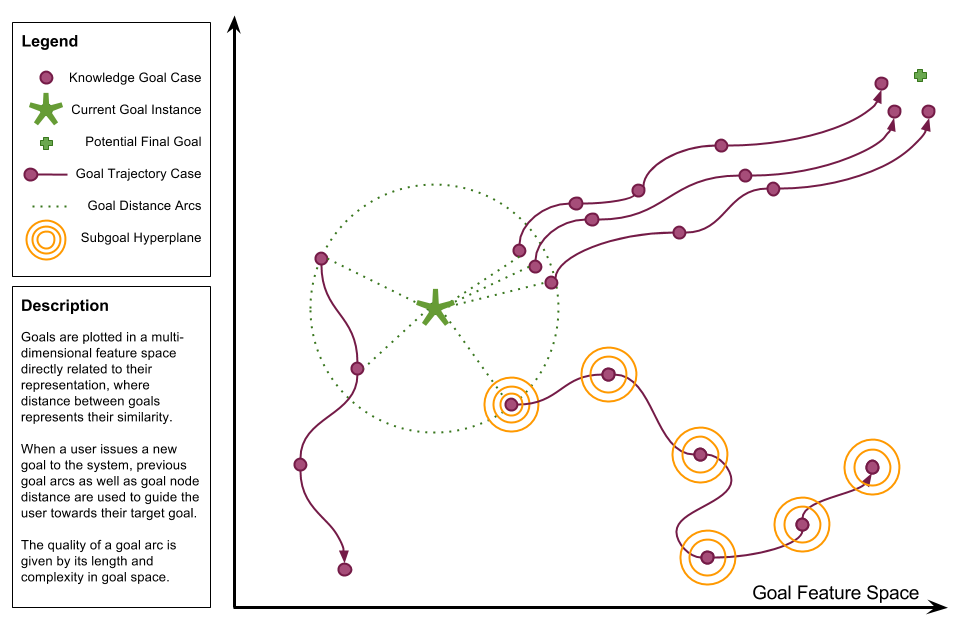
\includegraphics[width=0.75\textwidth]{figures/representation.png}
\caption{\label{fig:representation}A representation of the knowledge goal dimensional space. Each goal is a point in this space, and a trajectory is a path through knowledge goals. A user is accelerated if they can be guided to or through a similar goal trajectory, skipping over unnecessary goals. A user short-circuits dead ends or tangents in complex knowledge goals by maintaining a vector towards the final point in the followed trajectory.}
\end{figure} 

\subsection{Knowledge-Goal Space}

The goal space is a multidimensional representation of all possible knowledge goals where a point in this space is a goal location. Similar knowledge goals should therefore be close as measured by geometric distance. The goal vector space is created by features of the natural language question that represent the \textit{concept}, \textit{context}, and \textit{task}. In particular, each of these components of the knowledge goal representation is a unique vector that is unioned with the other three components to form the complete vector.

\begin{enumerate}
    \item \textbf{Concept Vector}: The concept vector uses a \textit{Term Frequency Inverse Document Frequency} (TF-IDF) vector of the words in the question. Because questions are so short, TF-IDF is a good measure of the importance of infrequent words in the corpus. Moreover, this vector is reduced by a truncated singular value decomposition (SVD) such that only the 50 best components of the vector remain.
    \item \textbf{Task Vector}: We have identified 9 potential task related to why the knowledge goal is being solved including factual questions like ``who'' or ``what'', explanation questions like ``why'' or ``how'', as well as existential and permission tasks. This vector is simply a boolean vector of the tasks of these questions based on a lightweight syntactic analysis.
    \item \textbf{Context Vector}: The context vector embeds user specific information into the goal including time of day, location of query, as well as relative position of the knowledge goal in a dialogue.
\end{enumerate}

These component vectors are easily computed from a natural language question using a lightweight parsing technique. The final knowledge goal representation is simply the ordered union of the concept, task, and context vectors. Because the TF-IDF vector in particular has to be computed on a medium to large corpus of questions ahead of computing the vector at run time, three corpora were used: \textit{Free917}, WebQuestions, and Kyudo. The distribution of questions from this corpus is shown using a principle component analysis (PCA) of the two most informative directions of each dimension, then mapped to two dimensions as shown in Figure \ref{fig:shaku_clusters_pca}.

\begin{figure}{}
\centering
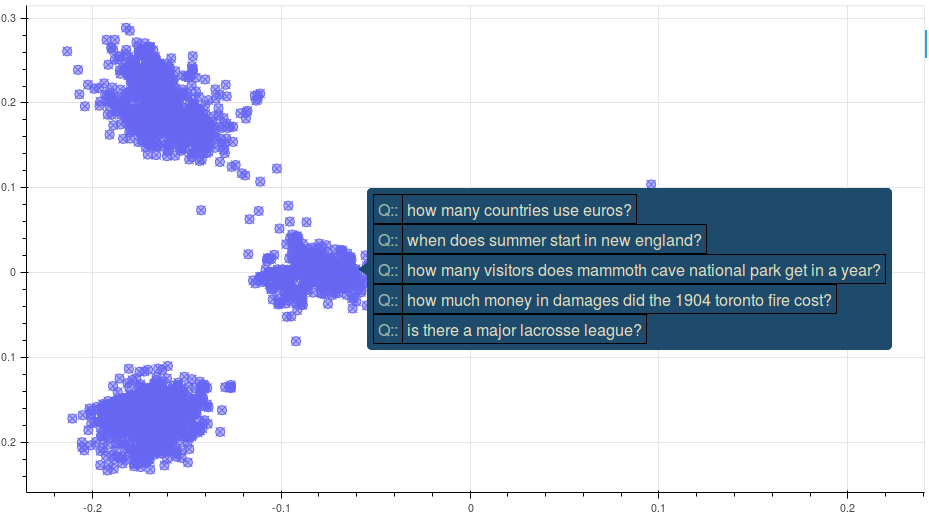
\includegraphics[width=0.75\textwidth]{figures/shaku_pca_nh.png}
\caption{\label{fig:shaku_clusters_pca}PCA projection of knowledge goals from the \textit{Free917}, \textit{WebQuestions}, and \textit{Kyudo} corpus of knowledge goals. Note that distinct clusters have formed, generally related to task. The menu showing questions at the cursor point uses the k-nearest neighbor algorithm to dynamically enumerate the list interactively.}
\end{figure} 

\subsection{Similarity Retrieval}

For each new Knowledge Goal or question posed to Kyudo, the parser produces a grammatically structured parse tree of constituent phrases. Each token from the phrase is queried to Wikipedia to fetch the related semantic entities from the first section of the page. This extract is filtered for stop words and we calculate the (TF-IDF) measure over all the knowledge goals we have in the case base. This provides an addition to Kyudo's corpus to expand Kyudo's knowledge of semantically related keywords and therefore any conceptually related knowledge goal in Kyudo's database.

\begin{figure}{}
\centering
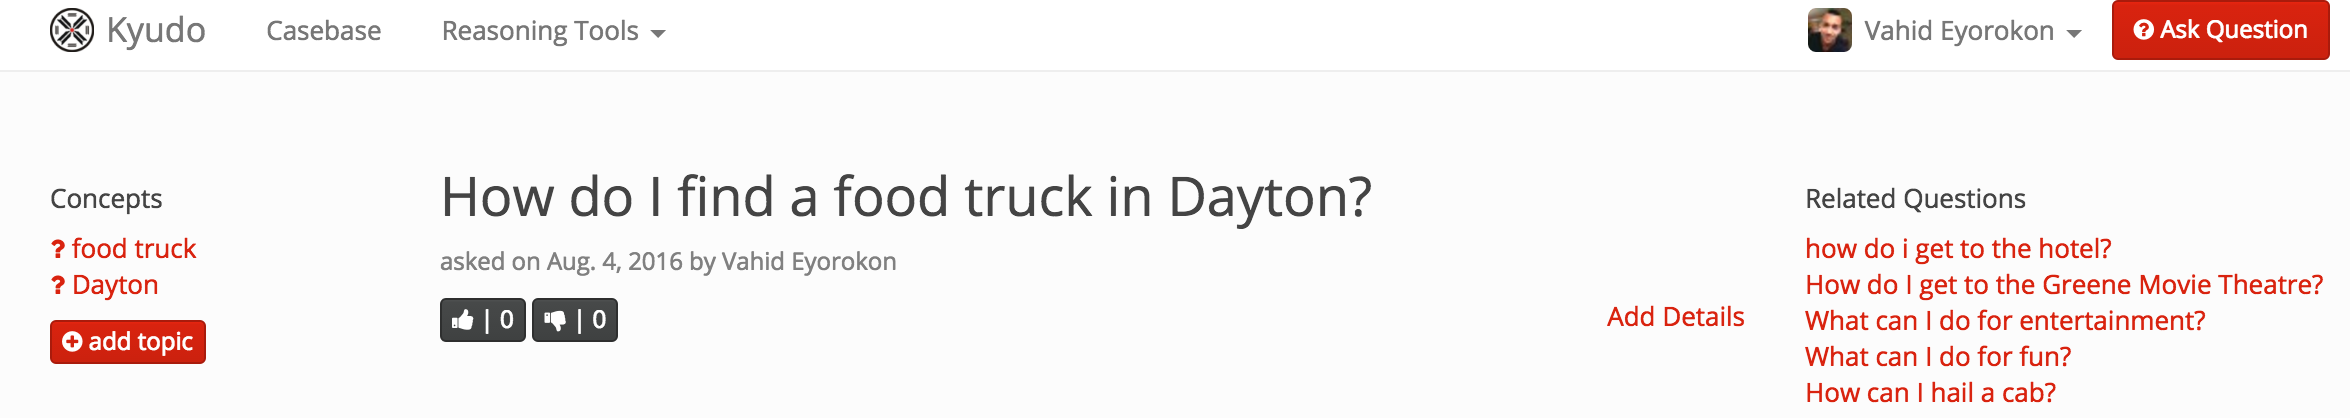
\includegraphics[width=0.75\textwidth]{figures/question.png}
\caption{\label{fig:kyudo_tfidf_similarity}Kyudo application showing the related questions fetched for the natural language question asked.}
\end{figure} 

A weight is assigned to each of the three components, i.e., concept, context and task of the question.  The responses retrieved for a question with a greater weight on context would fetch more related questions matching the context metadata rather than matching either task or concept related keywords. Figure \ref{fig:kyudo_tfidf_similarity} shows the retrieved similar questions based on the method discussed above.


\section{Goal Trajectory Retrieval}
	Kyudo's Reasoner interface shown in Figure \ref{fig:kyudo_interface}, engages the user in a conversation where the user asks a series of questions or knowledge goals specifying whether each one is a new goal or a sub-goal. The series of knowledge goals asked becomes a dialogue or goal trajectory and is used to retrieve similar goal trajectories from Kyudo's case base.
	Retrieval is based on: concept, context and task. For each new goal trajectory initiated by a user, Kyudo will first retrieve all stored cases of goal trajectories that pass contextual checks of time and profile similarity based on k-nearest neighbors algorithm. In the time check, the start times for each retrieved case is compared to the start time of the new goal trajectory. If the time difference is less than an arbitrary threshold of 4 hours, the goal trajectory \textit{survives} and will then be processed for profile similarity. Profile similarity will then check the similarity of the user in the new goal trajectory against users in all surviving goal trajectories for matches in gender, marital status, and an age difference within an arbitrary threshold of 4 years. If the processed goal trajectory matches in at least 2 of these 3 attributes, the goal trajectory survives to be processed by the final check of initial similarity.
    
\begin{figure}[!t]
	\centering
    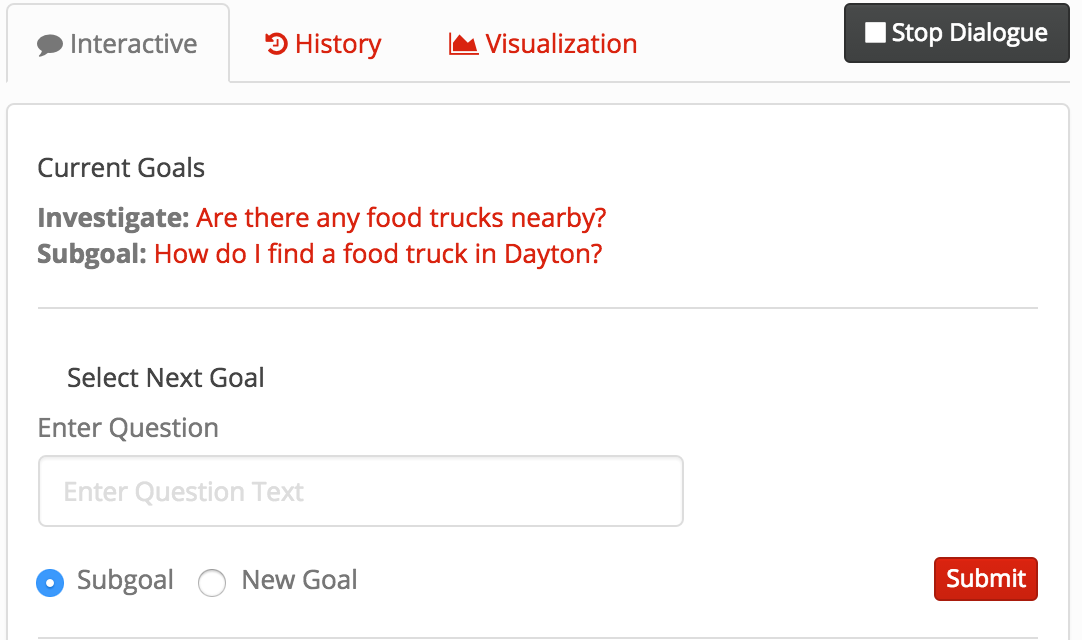
\includegraphics[width=0.75\textwidth]
    {figures/interface.png}
    \caption{Kyudo's reasoner application interface.}
    \label{fig:kyudo_interface}
\end{figure}

\subsection{Initial Similarity Check}
The \textit{Initial Similarity Check} measures task and conceptual relevance of the knowledge goals that appear in the beginning of each surviving goal trajectory against the knowledge goals in the current goal trajectory whose length is $n$. For each knowledge goal that appears in the current goal trajectory, the top 5 TF-IDF related knowledge goals are calculated. This extends Kyudo's matching beyond simple exact text matches and allows for matches with conceptually related questions. 
	
    A list $l$ is created containing all knowledge goals in the current goal trajectory and their conceptually relevant goals as determined by the TF-IDF measures while omitting duplicates. Kyudo then compares up to the first $n$ number of goals in each of the surviving goal trajectories, against all goals in list $l$ to calculate the number of initial similarity matches.

    If the number of initial similarity matches for a particular goal trajectory is greater than or equal to a set threshold of $n$/2, then the goal trajectory is considered a match and survives. All surviving goal trajectories are then ranked by their number of initial similarity matches and the id for the dialogue with the greatest number of matches is returned. 

\section{Related Research}
This work is related to \cite{powell_2011} which demonstrates a case-based reasoning approach to the adaptation of knowledge which can be dynamically mined from web-based resources. Their novel method utilizes large web-based data sets, similar to Wikipedia used by Kyudo, in order to solve the problem of adaptation or revision of a case to make it applicable to the user's current task. Our work with Kyudo adopts a similar web-based data mining approach and incorporates dialogues which track the overall sequence of goal changes and the evolution of the questions \cite{ram_1991} being asked. Our work differs in that goal changes, along with the addition of conceptual knowledge and contextual relevance, allow Kyudo to retrieve not just related questions, but entire dialogues. While their work improves their systems ability to adapt cases, our work focuses more on tracking the goal changes within the current dialogue thereby allowing Kyudo to guide the user's current investigation based on our case base and short circuit the user's knowledge discovery process.
	
	Our approach builds upon previous work \cite{bengfort_interactive_2015}, particularly a taxonomy of knowledge goals,  to create a multidimensional representation of a knowledge goal. This representation is defined by a knowledge goal space with which we can compare goal similarity using distance metrics. This implementation therefore allows us to use lightweight and fast nearest neighbors algorithms to provide guidance to the user; a simplification that improves upon many challenges regarding case-based learning.

	The work of \cite{aha_advances_2005} is highly relevant due to Kyudo's conversation based interface. Their work highlighted the importance of refining the user's question in order to solve a problem. Such problems faced by the user are usually vaguely or briefly defined and lack adequate detail for the system to provide a meaningful solution. Their method of implementing a conversational style interface to extracting details of a target goal was proven to be effective and close to the natural way humans communicate problems. Our work builds on this style of conversation based interface and also tracks the user's decomposition of goals into sub-goals. By allowing users to map out a 'plan' to solve their target goal, Kyudo can better understand the context of why goals change and identify false tangents to better provide guidance.
    
    The research described in \cite{cox_mixed-initiative_2007} emphasizes the need for systems with the potential to maximize the individual strengths of humans and AI. Their work argues the need to 'model planning as a goal-manipulation task' or mixed-initiative planning as opposed to traditional search based planners. Mixed-initiative planning regards plans as being a series of goal adaptations \cite{cox_goal_1998} and this overall evolution as being the byproduct of human and AI collaboration. Goal transformation and goal reasoning as discussed in \cite{cox_dannenhauer} plans for the goals using metacognition. 
    
	Kyudo's Reasoner application engages the user in a dialogue and through a series of knowledge goals, the user provides Kyudo with the general trajectory the dialogue takes. As the dialogue progresses, Kyudo's understanding of both the target goal and retrieval improves which enhances \cite{ram_1990} its ability to guide the direction of the conversation and streamline the user's knowledge discovery process. The dialogue itself then becomes a plan with the goal being for the user to obtain a solution to the target goal of their investigation.
    
    The work done in \cite{lopez_de_mantaras_retrieval_2005} has proven to be invaluable as it succinctly describes the overall architecture of any case-based reasoning system. In their paper, they describe retention, reuse, revision and retrieval as being the main components of a case-based reasoning system. Kyudo adheres closely to their methodology which has provided a framework from which Kyudo was modeled. By providing our team with the terminology necessary for effective communication, the process of Kyudo's development has proven to be more practical.
    
\section{Conclusion}

Knowledge investigations made by humans often follow different trajectories based on the target goal of their investigation. By providing guidance towards a target knowledge goal, Kyudo accelerates the user’s investigation process and helps to avoid false tangents. Our work represents a knowledge goal as a vector comprising of concept, context and task components. Kyudo incorporates Case-based reasoning principles for goal retrieval by calculating the TF-IDF of the given natural language question to expand it's own knowledge by fetching the related semantic entities from Wikipedia. This enables Kyudo to provide the user with more accurate information vital to achieve successful knowledge discovery and retrieve matching goal trajectories. Current work is being done to further develop Kyudo's guidance capabilities and recognition of false tangents within a dialogue. Adaptation of related dialogues has yet to be developed and is another area of future research.

\section{Acknowledgments}
This work was supported in part by ONR under grants N00014-15-1-2080 and N00014-15-C-0077. We thank the anonymous reviewers for their comments.


%
% ---- Bibliography ----
%
\begin{thebibliography}{5}
%
\bibitem {aha_advances_2005}
Aha, D. W.; McSherry, D.; and Yang, Q. 2005. Advances
in conversational case-based reasoning. The knowledge engineering review 20(03):247–-254

\bibitem {bengfort_interactive_2015}
Bengfort, B., Cox, M. T. (2015). Interactive reasoning to solve knowledge goals. In D. W. Aha (Ed.), Goal reasoning: Papers from the ACS workshop (pp. 10--25). Tech. Rep. No. GT-IRIM-CR-2015-001. Atlanta, GA: Georgia Institute of Technology, Institute for Robotics and Intelligent Machines.

\bibitem {berant_semantic_2013}
Berant, J.; Chou, A.; Frostig, R.; and Liang, P. 2013. Semantic Parsing on Freebase from Question-Answer Pairs. In
EMNLP, 1533-–1544.

\bibitem {cox_goal_1998}
Cox, M. T., and Veloso, M. M. 1998. Goal transformations
in continuous planning. In Proceedings of the 1998 AAAI
fall symposium on distributed continual planning, 23–-30.

\bibitem {cox_mixed-initiative_2007}
Cox, M. T., and Zhang, C. 2007. Mixed-initiative goal manipulation. AI Magazine 28(2):62.

\bibitem {kolodner_case-based_1993}
Kolodner, J. 1993. Case-based reasoning. San Francisco: Morgan Kaufmann.

\bibitem {lopez_de_mantaras_retrieval_2005}
Lopez De Mantaras, R.; McSherry, D.; Bridge, D.; Leake,
D.; Smyth, B.; Craw, S.; Faltings, B.; Maher, M. L.; Cox,
M. T.; Forbus, K.; and others. 2005. Retrieval, reuse, revision and retention in case-based reasoning. The Knowledge
Engineering Review 20(03):215–-240.
\bibitem{powell_2011}
Powell, J. 2011. A generic web-based discovery framework for case-based reasoning. Ph.D. Dissertation, Indiana University, Computer Science Department, Bloomington, IN.
\bibitem {wang_wisdom_2013}
Wang, G.; Gill, K.; Mohanlal, M.; Zheng, H.; and Zhao,
B. Y. 2013. Wisdom in the social crowd: an analysis of
quora. In Proceedings of the 22nd international conference
on World Wide Web, 1341–-1352. International World Wide
Web Conferences Steering Committee.

\bibitem {yahya_natural_2012}
Yahya, M.; Berberich, K.; Elbassuoni, S.; Ramanath, M.;
Tresp, V.; and Weikum, G. 2012. Natural language questions
for the web of data. In Proceedings of the 2012 Joint Conference on Empirical Methods in Natural Language Processing
and Computational Natural Language Learning, 379–-390.
Association for Computational Linguistics.

\bibitem{ram_1990}
Ram, A. (1990). Knowledge goals: A theory of interestingness. Proceedings of the Twelfth Annual
Conference of the Cognitive Science Society (pp. 206–-214).

\bibitem{ram_1991}
Ram, A. (1991). A theory of questions and question asking. Journal of the Learning Sciences, 1,
273–-318.

\bibitem{cox_dannenhauer}
Cox, M. T., Dannenhauer, D. (2016). Goal transformation and goal reasoning. In Proceedings of the 4th Workshop on Goal Reasoning. New York, IJCAI-16.
\end{thebibliography}

\end{document}


